\documentclass[tikz,border=10mm]{standalone}
\usepackage{amsmath}
\usepackage{amsfonts}
\usepackage{amssymb}
\usepackage{pgfplots}
\pgfplotsset{compat=1.18}

\begin{document}
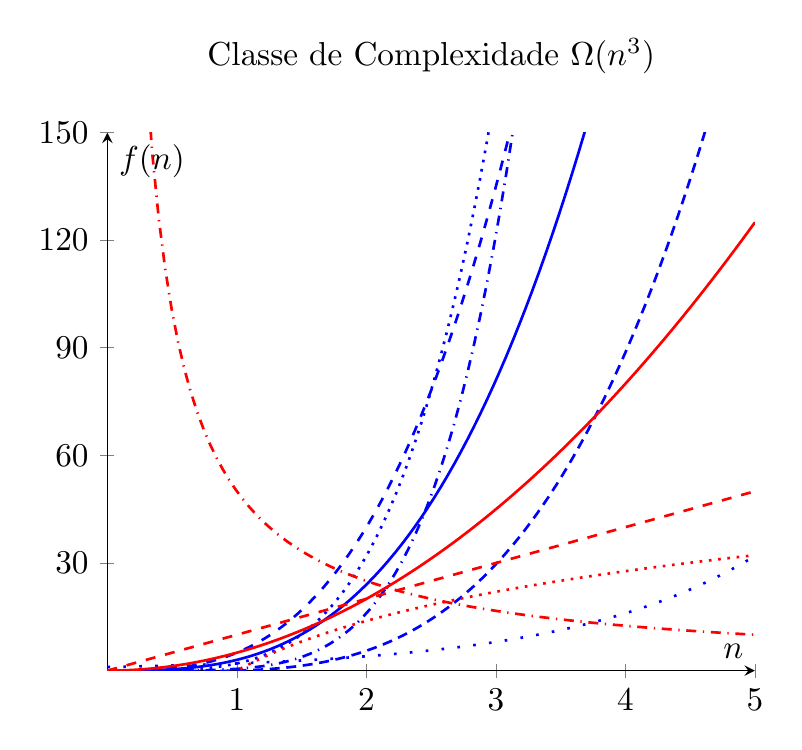
\begin{tikzpicture}[scale=1.2]
\begin{axis}[
    xlabel={$n$},
    ylabel={$f(n)$},
    axis lines=middle,
    xmin=0, xmax=5,
    ymin=0, ymax=150,
    xtick={1,2,3,4,5},
    ytick={0, 30, 60, 90, 120, 150},
    title={Classe de Complexidade $\Omega(n^3)$},
    title style={at={(0.5,1.05)},anchor=south}
]
\addplot[blue, thick, domain=0:5, samples=100] {3*x^3};

\addplot[blue, dashed, thick, domain=0:5, samples=100] {5*x^3};

\addplot[blue, dotted, thick, domain=0:5, samples=100] {2*x^4};

\addplot[blue, dashdotted, thick, domain=0:5, samples=100] {0.5*x^5};

\addplot[blue, densely dashed, thick, domain=0.1:5, samples=100] {x^3*ln(x)};

\addplot[blue, loosely dotted, thick, domain=0:5, samples=100] {2^x};


\addplot[red, thick, domain=0:5, samples=100] {5*x^2};

\addplot[red, dashed, thick, domain=0:5, samples=100] {10*x};

\addplot[red, dotted, thick, domain=0.1:5, samples=100] {20*ln(x)};

\addplot[red, dashdotted, thick, domain=0.1:5, samples=100] {50/x};


\end{axis}
\end{tikzpicture}
\end{document}
